\renewcommand\thetable{\arabic{chapter}-\arabic{table}}
%\renewcommand\thefigure{\arabic{chapter}-\arabic{figure}}
\renewcommand{\theequation}{\arabic{chapter}-\arabic{equation}}
\chapter{資料探勘}

過往在各種不同商業、工業、學術等領域都隨著產業逐步的數位化,有各種資料庫甚至資料倉儲系統的建置與資料收集,例如零售業的交易紀錄,各種學術實驗的結果記錄等等,而隨著時間推移,這些資料庫和倉儲系統收集的資料數量都成長的非常龐大,資料間的關係和複雜度也越來越複雜,這些資料除了當初建置的目的和資料的統計分析外,研究人員還開始思考更進一步的資料應用,希望能把資料中以往隱藏不可見的知識找出來,因此資料探勘(data mining)此一研究領域就因應而生。應用在資料探勘研究的演算法非常多種,包括統計、線上分析處理(OLAP、on-line analytical processing)、情報檢索(information retrieval)、機器學習(machine learning)、模式識別(pattern recognition)等,只要能夠用來在大量資料中尋找有資訊的方法,都可以作為資料探勘的演算法。

資料探勘的流程也有多種規範,其中最廣為被使用的是~CRISP-DM\cite{shearer2000crisp}(Cross Industry Standard Process for Data Mining),是由~SPSS~以及~NCR~兩大廠商在~1990年開始發展的,它的流程架構如圖~\ref{fig:CRISP-DM}~所示,將一個完整的資料探勘流程分為六個步驟,分別為:

\begin{figure}[hbtp]
  \begin{center}
    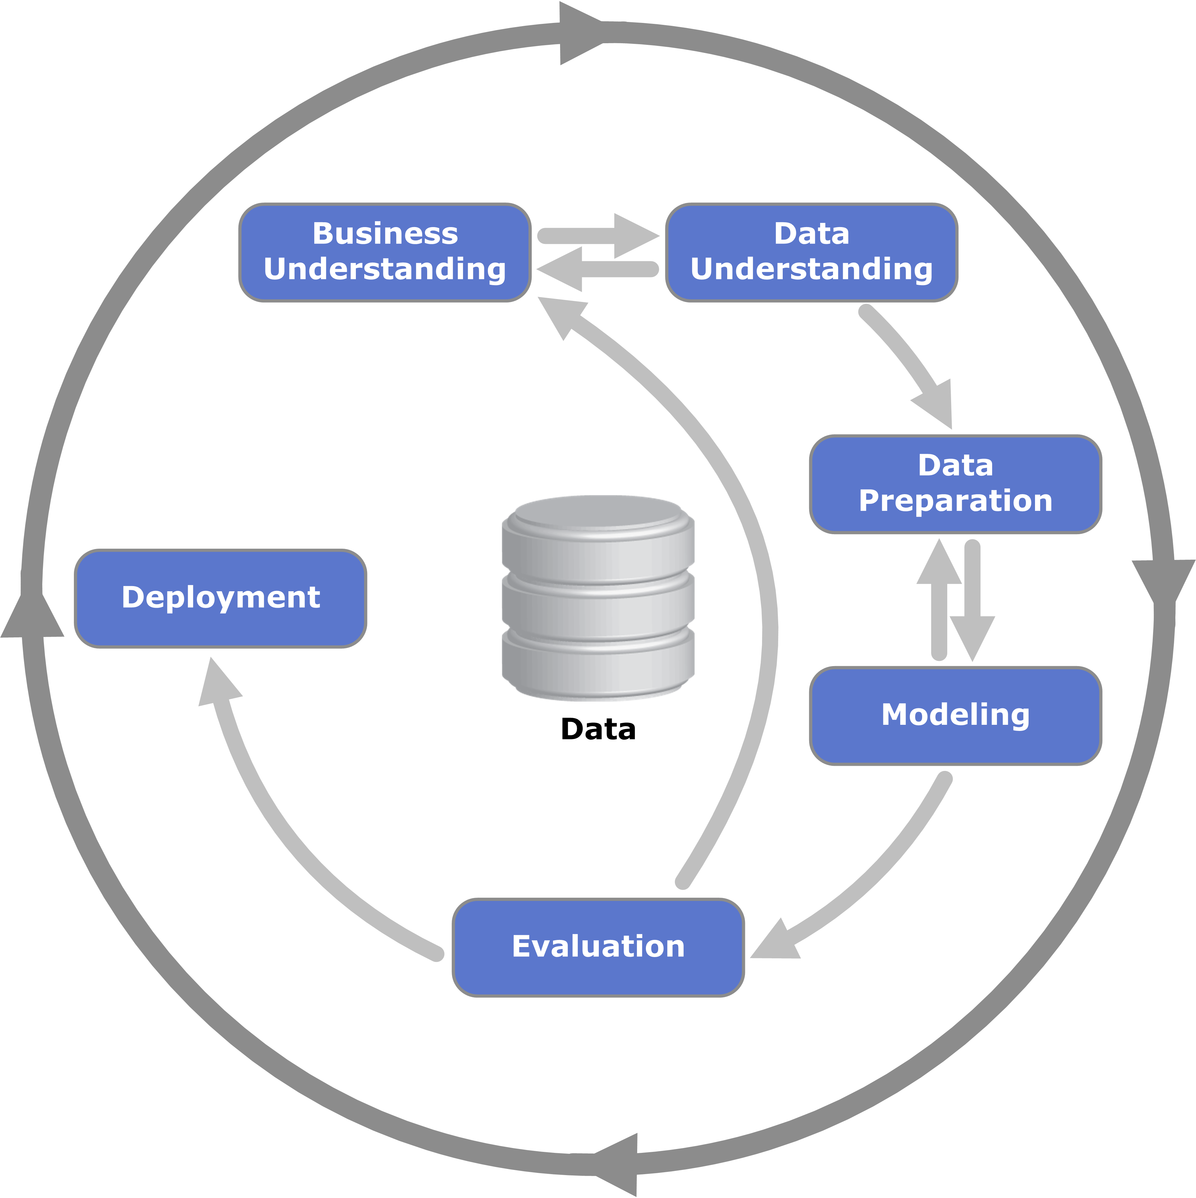
\includegraphics[width=1.0\textwidth]{figures/1196px-CRISP-DM_Process_Diagram.png}
    \caption{CRISP-DM 流程圖 (c)Kenneth Jensen, CC BY-SA 3.0} 
    \label{fig:CRISP-DM}
  \end{center}
\end{figure}

\begin{enumerate}
\item \textbf{定義領域問題}(Business Understanding),CRISP-DM~所定義的資料探勘最初的步驟是瞭解並定義此一資料探勘所希望解決的問題。
\item \textbf{定義分析資料}(Data Understanding),瞭解問題之後,就要定義要解答此一問題所需要的資料為何,並且著手收集。
\item \textbf{資料前處理}(Data Preparation),這個步驟包括了資料的由於現實世界的資料都會有很多雜訊在其中,因此在真正的訓練並建立模型之前,需要先把雜訊去除,包括了不合理的資料、多餘欄位,甚至是透過一些方法來凸顯資料中本來較不明顯的特定性質。
\item \textbf{建立模型}(Modeling),選擇適合該問題的資料探勘方法對前處理過的資料進行分析與模型建立。
\item \textbf{評估模型}(Evaluation),評估前一步驟中所建立的模型品質是否符合需,多是將資料分為訓練集與測試集兩組來驗證模型的可靠度。
\item \textbf{應用模型}(Deployment),將模型產出的知識實際納入應用,抑或是將探勘結果整理成完整的報告。
\end{enumerate}

本研究之流程較~CRISP-DM~之流程稍有不同,是先基於一個現有的特定領域的校舍耐震資料庫作分析,找出校舍耐震資料庫中各種潛藏知識的可能性,定義出希望能夠解決的問題,接著分析不同的問題,從校舍耐震資料庫中挑選出相關的資料屬性,然後接著進行資料前處理、建立模型、評估模型幾個步驟。

資料探勘技術方法繁多,Fayyad~\cite{fayyad1996data}根據其處理的問題形式,將資料探勘的方法分為分類、分群、迴歸尋找關聯等四種主要的問題類型。其中,分類方法處理的問題是在用來判斷資料的類別,而且這些類別是已知的類別,例如將所有的校舍資料分類成有安全疑慮和沒有安全疑慮的就是屬於分類問題。分群問題和分類問題有點相似,一樣是將資料分成數個群組,最主要的差異是分群問題的各個群組特性一開始並不清楚,分群方法是將資料根據其屬性數值為依據,把相似的放在同一個群組,不同群組的特性是要在分出群組後進行分析才會得到。迴歸問題就是要用回歸方法來從資料的屬性中,找出特定屬性與其他屬性間的關係模型,這些屬性間的關係可能是非線性的,而且沒有解析解的關係模型,因此常見的方法是用統計回歸的方式,用現有的資料來回歸得到,又或著是用像類神經網路之類的機器學習方式,拿現有的資料下去學習已得到關係模型,以校舍耐震資料庫來說,校舍耐震能力指標的預測就是一種回歸問題,因為校舍耐震能力指標與其校舍的設計參數間的關係就是一個非線性關係,要得到兩者之間的非線性模型就需要用到回歸問題的處理方法,回歸問題也是最常見的資料探勘問題種類。最後一種是尋找屬性間的關聯,這種問題的主要目標在尋找不同筆資料屬性間所存在的關係,舉例來說,使用校舍耐震資料庫的資料來作關聯分析,可能可以去尋找像是:五層樓的校舍的校舍長度深度有什麼趨勢,或是民國八十到九十年之間的校舍的校舍走廊設計是否偏好有走廊柱等。本研究在確定主要的探勘目標後,使用的資料探勘方式為迴歸為主,分類分群為輔助。

以下分別介紹本研究所使用到的各種分析方法,除建立模型的各種訓練和學習演算法外,還包括資料前處理和驗證所使用的分析方法和驗證指標。


\section{資料前處理方法}

資料前處理方法常見的目的有:找出重要性較高的屬性、凸顯資料特性、剔除特異資料點等;本研究主要的資料過濾方法為資料的合理性分析,其是根據資料特性,根據經驗與專家意見等參考依據,建立出資料合理性的判斷方法。而除了合理性分析外,尚有較為簡單的數種方法,包括:

\begin{itemize}
\item 輸入屬性篩選
\item 子資料集挑選
\end{itemize}

剩餘有較複雜的數學理論背景的前處理方法,只有主成分分析法。

\subsubsection{主成分分析}

主成分分析(Principal Component Analysis,PCA)是常見的前處理方法,它可以用來減少資料的維度,其數學原理是將資料向量投影到不同的座標系統,將原始的資料轉換成不同座標系的的向量資料,且能保持最大程度的,輸入屬性對於輸出屬性的貢獻。

% PCA, a very common data preparation method, can identify very important attributes among various attributes. The goal is to convert the original variables through vector transition into mutually independent variables of a linear combination. The ideal situation is that principal components obtained from linear combination retain most of the information of original variables.

\section{資料探勘方法}

資料探勘的方法分為分類、分群、迴歸以及尋找關聯~\cite{fayyad1996data}~,其中迴歸是最常使用到的一種,本研究的主要目標皆可以歸納為迴歸類的問題,因此使用到的迴歸演算法最多,接著才是作為輔助用的分類和分群演算法。

迴歸、分類、分群三種資料探勘所建立的模型可以簡單的定義為:

\begin{equation} y = f(x) \label{eq:ModelEqu}\end{equation} 

$f(.)$~就是透過資料探勘分析學習而得到的模型函數,~$x$~代表輸入參數,輸入參數是各種已知的屬性資料,例如可以簡單透過量測得到的校舍尺寸資訊,~$y$~則是代表輸出參數,也就是希望透過這個模型所得到的,比較難取得的屬性資料,例如需要經過詳細評估才能的到的校舍~$CDR$~值、或是校舍分類的類別索引。

\subsection{迴歸方法}

\subsubsection{Generalized Linear Model}

廣義線性模型是由Nelder and Wedderburn~\cite{citeulike:5485398}所提出,比起迴歸分析(simple regression)更為彈性,此模型是假設資料點的分佈有一分佈模式,且輸入參數~$x$~與輸出參數~$y$~之間的關係是由一連結函數(Link Function)建立,如~log function、power function~等,其定義之~$x$~與~$y$~間之關係模型如下:


\begin{equation} g(E(y)) = x\beta + O, y \sim F \label{eq:GLM}\end{equation} 

$g(.)$是為所選的鏈結函數,~$O$~是偏移(offset)變數,~$F$~則是~$y$~的分佈模型,其是用牛頓法(Newton-Raphson Method)不斷的調整~$\beta$~使的~$x\beta + O$~逼近~$g(E(y))$~,最後最接近的方程式即為~$x$~與~$y$~兩者的關系式。比起迴歸分析,此方法還需要了解~$y$~值分佈狀況,選擇出最適合的分佈函數,並假設~$x$~與~$y$~間的鏈結函數形式,雖然越多的參數選擇代表了更多的模型不確定性,但廣義線性模型卻能夠提供比迴歸分析更廣的應用範圍,也可能得到更接近真實的關係模型。


\subsubsection{類神經網路}

類神經網路(Artificial Neural Networks,ANNs),其是希望能模擬建構出人腦內的神經網路,以處理各種複雜的問題,人類大腦是由大約千兆個神經元(Neuron)所構成,而每個神經元又會和其他約一萬個神經元連結,構成一個龐大且複雜的神經網路,這樣複雜的一個神經網路讓人類可以學習並了解各種事物與知識。McCulloch and Pitts~\cite{mcculloch1943logical}所提出的模型為後續類神經網路發展的雛形,而目前最為被廣反使用的類神經網路結構為倒傳遞類神經網路(Back-Propagation Network, BPN),為一種監督式學習網路,應用十分廣泛。Werbo~\cite{werbos1974beyond}首先提出隱藏層及倒傳遞學習理論的概念,但在當時並未受到重視。直到~Rumelhart~及~McClelland\cite{rummelhart1986learning}於~1986~提出~BPN~學習演算法及通用差距學習法則(Generalized Delta Learning Rule),採引起學者的廣泛討論。倒傳遞演算法是將一組樣本~1/0~問題變為一個非線性最佳化的問題,其基本原理是利用最陡梯度下降法(Gradient Steepest Descent Method)以計算且調整網路權重,使推論輸出值與目標輸出值間的誤差最小化,得到精確的學習。因此,倒傳遞類神經網路是用於診斷與預測上,若將此模式視為輸入與輸出間的映射關係,則~BPN~演算法是一種輸入輸出的映射過程,一個標準的~BPN~類神經網路可以分為輸入層(input layer)、隱藏層(hidden layer)、輸出層(output layer),其結構如圖~\ref{fig:ANN-network},分別介紹三種神經元如下:

\begin{description}
  \item [輸入層神經元]
  用以表現網路的輸入變數,其處理單元數目依問題而定,通常相等於所使用的輸入參數,使用線性轉換函數,即~$f(x)=x$。
  \item [隱藏層神經元]
  用以表現輸入處理單元間的交互影響,其處理單元數目並無標準方法可決定,經常需以試驗方式決定其最佳數目,使用非線性轉換函數,網路可以不只一層隱藏層,也可以沒有隱藏層。
  \item [輸出層神經元]
  用以表現網路的輸出變數,其處理單元數目依問題而定,使用非線性轉換函數。
\end{description}

\begin{figure}[hbtp]
  \begin{center}
    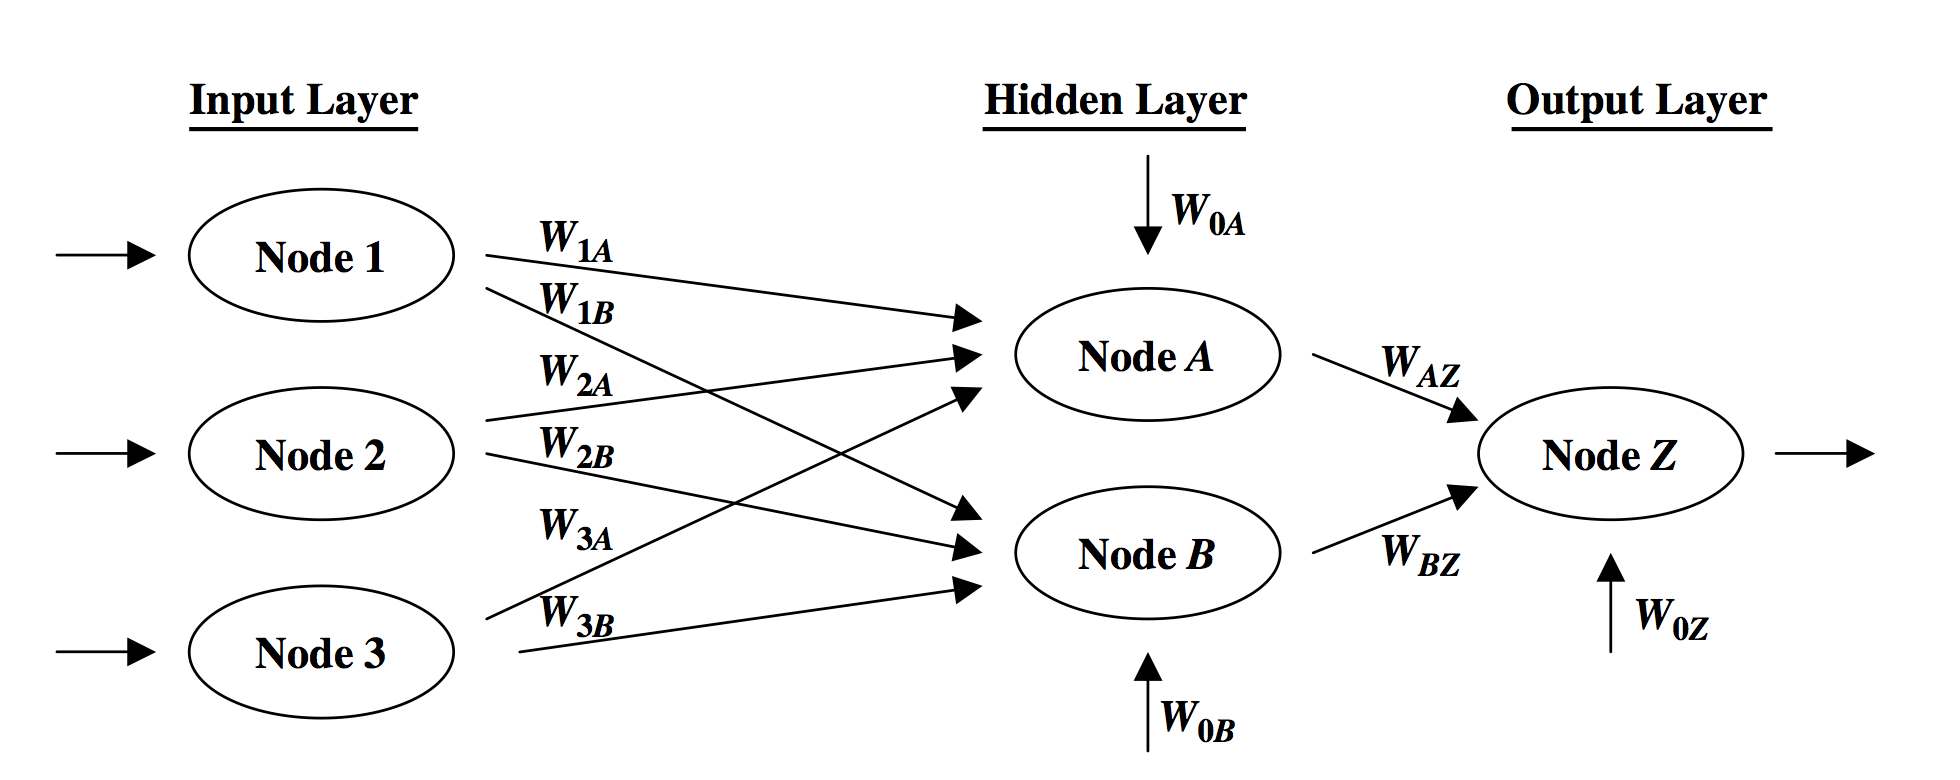
\includegraphics[width=1.0\textwidth]{figures/anns-network.png}
    \caption{類神經網路結構圖~\cite{larose2005discovering}} 
    \label{fig:ANN-network}
  \end{center}
\end{figure}

處理單元其輸出值及輸入值的關係式,一般可用輸入值的加權乘積和之函數來表示:

\begin{equation}\begin{split}  Y_j &= f(net_j) \\ net_j &= \sum W_{ij}X_i - \theta_j \label{eq:anns}\end{split}\end{equation} 

其中,$Y_j$~為輸出層第~$j$~個處理單元之推論輸出值,$net_j$~為輸出層第~$j$~個處理單元之集成函數,$W_{ij}$~為第~$i$~個輸入層單元與第~$j$~個輸出層單元間之連結權重。$X_i$~為輸入層第~$i$~個處理單元之輸入值。$\theta_j$~為輸出層第~$j$~個處理單元之閥值,$f$~為轉換函數,是為神經元從輸入層加總轉換至輸出的一種映射規則亦是將非線性的影響導入網路中的一種設計。而轉換函數的選擇相當多, 本研究採用的轉換函數為對數雙彎曲函數,如下所示:

\begin{equation} f(x) = \dfrac{1}{1 + e^x}  \label{eq:annsf}\end{equation} 


\subsubsection{基因規劃}

基因規劃(Genetic Programming,GP)是基於基因演算法(Genetic Algorithm, GA)發展而來,而~GA~是~1975~年由~John Holland\cite{holland1975adaptation}~所提出的演化求解方法,其是基於生物演化的過程為基礎,假設問題的目標可以轉換為二元的基因序列,再透過模擬生物交配、突變的進化過程,求得最佳化問題的解,和傳統的演化求解方法相比,基因演算法可以比較容易的找到全域最佳解,且其可以快速的找到足夠好的解,即使問題的複雜度很高。基因演算法的應用領域相當廣泛,在營建領域也有不少的應用,Huang...et. al.\cite{minshui2009study}~就使用GA預測梁模型受力後會產生破壞的位置極其嚴重性,Šešok和Belevicius\cite{vsevsok2008global}~則使用基因演算法建立一個~truss topology~最佳化的建議系統。

基因規劃則是~1992~年由~Koza\cite{koza1992genetic}~所發表的方法,它是基於發展許久的基因演算法而來,將基因演算法所要演進發展的基因序列換為樹狀結構的分析樹(parse tree),並藉由與基因演算法相同概念的交配、突變和篩選等機制來達成解析樹的演化,並達成最佳化目標,如果要求得一數學關係方程式,則可以使用運算樹(operation tree)作為欲演進的解析樹結構。運算樹是一個二元樹結構,如圖~\ref{fig:GP-struct}~,其底層的末端點是方程樹的輸入變數或是其它常數、數值等,其餘的分支節點都是運算子(operator),藉由置換各個節點的輸入數值和運算子,就可以組成各種可能的數學方程式。此一方法的特色是其輸出即為輸入和輸出的關係方程式,且其方程式之形式不受限於基因演算法之特性。在營建領域使用~GP~加上運算樹進行最佳化的應用少有人做,Yeh and Lien\cite{yeh2009knowledge}~使用GP方法來預測混凝土強度。Tsai\cite{tsai2011using}~則使用修改過的~Weighted Genetic Programming~方法建立出~squat wall strengths~的方程式,並且還利用一些修剪公式的方法來調整得到的公式,讓公式可以更精簡,但是還保留有一定程度的可靠度。

\begin{figure}[hbtp]
  \begin{center}
    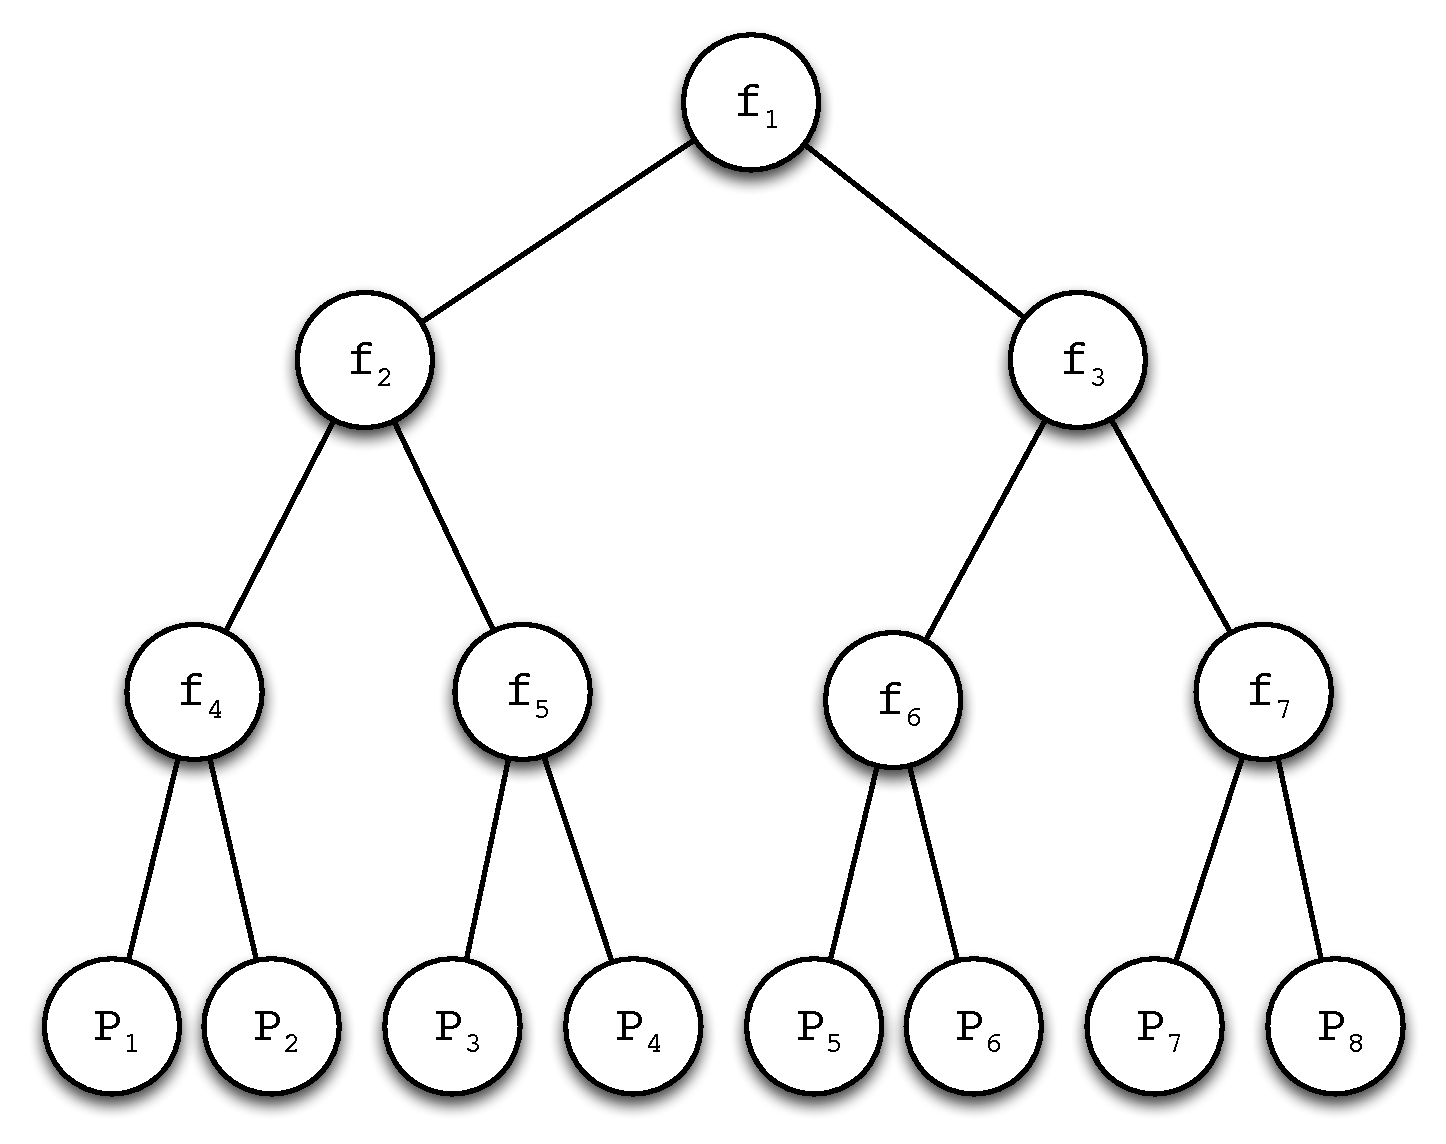
\includegraphics[width=1.0\textwidth]{figures/gp-struct.pdf}
    \caption{GP 運算樹結構示意圖} 
    \label{fig:GP-struct}
  \end{center}
\end{figure}

基因規劃藉由這樣的運算樹設計,再透過基因演算法最佳化輸入參數的選擇、不同運算節點的運算子,便可以根據資料建立出一個屬性與所求目標的關係方程式。

\subsubsection{加權基因規劃}

加權基因規劃(Weighted Genetic Programming,WGP)是由~Tsai\cite{tsai2011predicting}~所提出,基於~GP~ 方法發展而來,不同之處在於其運算樹的每個節點前都加上一個權重~$w$~,最佳化的過程除了對方程式結構和參數的選擇最佳化外,還要同時最佳化所有的權重,因此其輸出的關係公式可能性遠大於~GP~方法,故可以處理更為複雜的問題。~WGP~的運算樹結構如圖~\ref{fig:WGP-sample}~,每個運算樹都可以組成一個數學方程式,如圖~\ref{fig:WGP-sample}~之運算樹即可組成方程式如下:

\begin{equation} w_1(w_3(\dfrac{w_7P_2}{w_8P_6}) - w_4sin(w_9c))+w_2 \times cos(w_{12}c \times w_{11}P_1) \label{eq:WGP-sample}\end{equation} 


\begin{figure}[hbtp]
  \begin{center}
    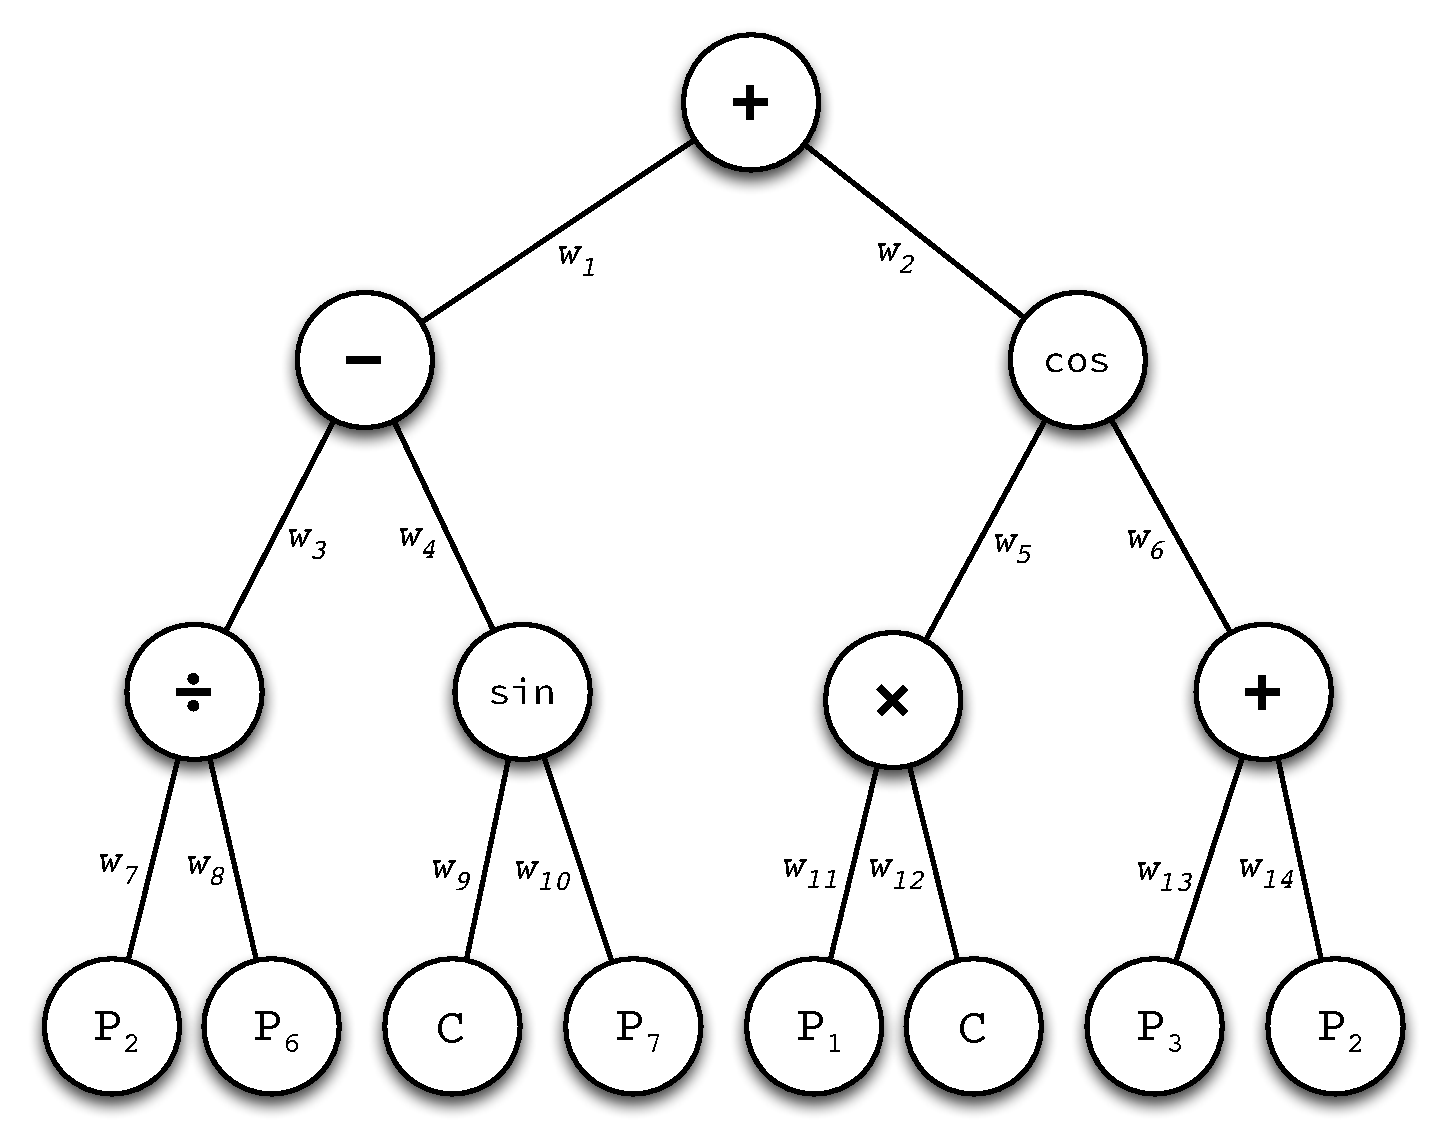
\includegraphics[width=1.0\textwidth]{figures/wgp-sample.pdf}
    \caption{WGP 運算樹結構示意圖} 
    \label{fig:WGP-sample}
  \end{center}
\end{figure}


運算樹可以分為兩種層級,運算層全部都是運算子節點,輸入層則是輸入參數的選擇,運算層每多一層,需要最佳化的節點和權重都會以等比例成長,運算層的層數也影響到最佳化結果的方程式複雜度,而輸入層則全部都是輸入節點,每層之間的每個連結都有一個權重參數,這些權重即為~WGP~方法最大的特色,這些權重可以讓運算樹組成的方程式有無限多種,也可以用以表示不同參數的重要性,因此雖然加入權重會讓最佳化更費時間,但仍然值得加上權重。

圖~\ref{fig:wgp-unit}~是一個構成~WGP~運算樹的基本單元,和圖~\ref{fig:gp-unit}~所示的~GP~運算樹的基本單元類似,包含一個父層節點和兩個子層節點,父層的節點是運算節點~$F$,透過權重參數連接到兩個子層節點,子層節點可能是其它的基本單元或是輸入節點,而整個基本單元的輸出~$y$~為:

\begin{figure}
  \begin{center}
    \subfigure[GP]{
      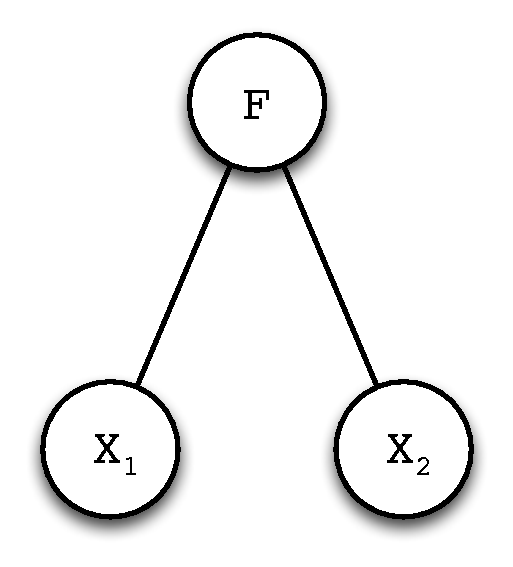
\includegraphics[width=0.4\textwidth]{figures/gp-unit.pdf}
      \label{fig:gp-unit}
    }
    ~
    \subfigure[WGP]{
      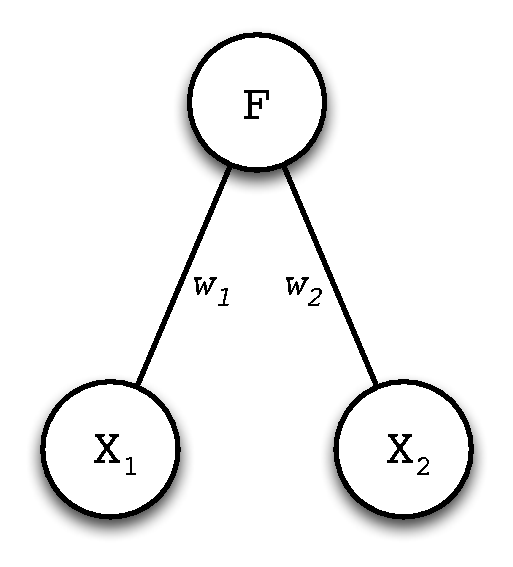
\includegraphics[width=0.4\textwidth]{figures/wgp-unit.pdf}
      \label{fig:wgp-unit}
    }
    \caption{GP 系統之單位元素}
    \label{fig:gps-units}
  \end{center}
\end{figure}

\begin{equation} y = \text{one of}\;\begin{cases}
  f_1 = w_1x_1 + w_2x_2 \\
  f_2 = w_1x_1 - w_2x_2 \\
  f_3 = w_1x_1 \times w_2x_2 \\
  f_4 = w_1x_1 \div w_2x_2 \\
  f_5 = \abs{w_1x_1}^{w_2x_2} \\
  \hphantom{f_1\;\;}\vdots \\
  f_n = \dfrac{1}{sin(w_1x_1)+cos(w_2x_2)}
\end{cases} \label{eq:WGP-y}\end{equation}

運算子~$F$~可能有數種選擇,同時配合最佳化演進得來的權重和子層節點的~$x_1$、$x_2$~,便可以計算得到這個基本單元的輸出~$y$,而子層節點的~$x_1$~和~$x_2$~有兩種可能的來源,一是此一基本單元的子層仍為運算層,則其數值要藉由計算該基本單元而來,另一種可能是子層為末端的輸入層,則~$x_1$~、~$x_2$~的值如下:

\begin{equation} x_i = \text{one of}\; \{1, P_1, P_2, P_3, \cdots P_j, \cdots P_{NI}\},\; j = 0 \sim NI \label{eq:WGP-xi}\end{equation}

其中~$NI$~為輸入參數的數量,$P_j$~為第~$j$~個輸入參數,$x_1$、$x_2$可能為輸入參數的任一個,$j = 0$~時為常數~$1$。

運算樹的層數~$NL$~定義為有運算節點的層數,即運算層的層數,運算樹的層數大小會影響到需要最佳化的基因數量~$N$,其公式為:

\begin{equation} N = 2^{NL} - 1 + 2^{NL} + 2^{NL + 1} - 2 = 2^{NL + 2} - 3  \label{eq:WGP-N}\end{equation}


其中運算層節點的函數選擇有~$2^{NL} - 1$~個、參數層的參數選擇有~$2^{NL}$~個、以及的權重~$w$~有~$2^{NL + 1} - 2$~個。藉由這樣的運算樹設計,再透過~GA~最佳化輸入參數的選擇、不同運算節點的運算子和各個節點不同的權重,~WGP~方法便可以根據資料建立出一個屬性與所求目標的關係方程式。

\subsection{分類方法}

\subsubsection{支撐向量機}

支撐向量機(Support Vector Machine,SVM)最早是BOSER~\cite{boser1992}等人,在~1992~年的~COLT(Computational Learning Theory)所提出,~SVM~是一個基於統計學習理論的分類方法,用來處理二元分割的問題,其原理是將原本無法線性分割的問題轉換到一個不同維度的空間(kernel)後,假設該空間存在一超平面(hyperplane),可以正確的將資料分開,並將尋找此一超平面的問題轉換為一最佳化問題,求解後即可得到二元分割邊界的方程式。而後~Harris Drucker, et. al.,\cite{drucker1997support} 將此二元分割問題轉換為迴歸分析問題,故~SVM~也可以處理迴歸問題。

\subsection{分群方法}

\subsubsection{K-means}

K-means~是由~MacQueen\cite{macqueen67}~所提出,也是最常被使用的分群演算法之一,屬於機器學習方法,其主要步驟為:

\begin{enumerate}
\item 使用者決定要將資料分為幾個群集,群集數為~$K$~。
\item 將資料隨機分到~$K$~個群組,並且計算出此時分群狀態下的每個群組的中心點。
\item 講每個資料點重新分群到新的群組,新群組的選擇方法為中心離它最近的那個群組。
\item 用新的分群狀態計算出新的群組中心點。
\item 重複步驟~3~和~4~直到每個資料點的群組都穩定不再變化。
\end{enumerate}


% As proposed by MacQueen~\cite{macqueen67}, K-means is one of the most common clustering methods and has a wide application scope. Notably, it is a machine learning method; its principal steps are as follows.


\subsubsection{兩步分群}

由於各種學術、商業研究所處理的問題資料量越來越大,分群演算法所需要的運算時間也急遽的成長,為了讓分群演算在處理大量的資料時也能有良好的效能表現,而發展出兩步分群法(Two-Step Clustering),其是由~Zhang~、~Ramakrishnan~與~Livny\cite{zhang1996birch}~所提出,此一方法分為兩個主要步驟:第一步是先把資料依據其與相鄰資料的相似度來排序並分成數個小群集,相似度的計算則是使用~log-likehood~函數,接著第二步再使用階層式分群方法,將這些群集慢慢組合或拆分直到達成停止條件。其特色在於運算複雜度較其他演算法來的低,例如~K-means~演算法就需要不斷的重複運算直到所有的資料歸屬都收斂不再變化為止,因此資料量成長時也不會讓運算時間成長到無法應用的程度。

% Based on of the massive volume of basic data for school buildings in the database, this study chooses two-step clustering method. The basic concept was first proposed by Zhang, Ramakrishnan and Livny~\cite{zhang1996birch} for handling large amounts of data. This method has two major steps. The first step sequences data and pre-clusters sequences into small subclusters based on the similarity of adjacent data, thereby reducing the amount of data. The second step divides several small subclusters into the desired number of clusters using a hierarchical clustering method. The hierarchical clustering method then combines close subclusters slowly until the stop condition is met. The computing speed of this method is influenced slightly by the volume of data.

%\section{探勘結果驗證方法與指標}
\section{探勘結果指標}

%\subsection{驗證方法}

%\subsubsection{10 fold cross validation}

%\subsection{結果指標}

\subsubsection{決定係數}

決定係數(coefficient of determination)又稱為~$R^2$~,其公式為:

\begin{equation} R^2 = 1 - \dfrac{SS_{res}}{SS_{tot}} = \dfrac{SS_{reg}}{SS_{tot}} = \dfrac{\sum{(\hat{y_i} - \tilde{y})^2}}{\sum{(y_i - \tilde{y})^2}} \label{eq:RSQ}\end{equation} 

其中 $y_i$ 是關係模型輸出屬性之值, $\hat{y_i}$ 則是該輸出屬性之實際值,$\tilde{y}$ 則是所有資料的輸出屬性實際值之平均,透過此一指標可以了解輸出屬性中有多少比例的資訊是由輸入屬性的變量所產生的,也代表著關係模型的正確性,而其值恰巧為關係係數~$R$(correlation coefficient)的平方,透過關係係數可以了解實際的輸出屬性數值與透過關係模型得到的推估值之間的線性關係,線性關係越高表示兩者之間越接近,也代表著關係模型所建立關係之正確性。

\subsubsection{平均絕對百分比誤差}

平均絕對百分比誤差(Mean Absolute Percetage Error, MAPE)~的公式如下:

\begin{equation} \text{MAPE} = \dfrac{\sum{\dfrac{\abs{y_i - \hat{y_i}}}{\hat{y_i}}}}{N} \times 100\% \label{eq:MAPE}\end{equation}

其中~$N$~是資料的總數,~$y_i$~是使用探勘得到的關係模型所求得的輸出屬性預測值,~$\hat{y_i}$~則是該屬性的實際值,此一指標代表了模型產出結果的平均誤差,可以呈現模型的準確度,數值越低代表模型品質越好。


\subsubsection{均方根誤差}

均方根誤差(Root Mean Squared Error, RMSE)定義如下:

\begin{equation} \text{RMSE} = \sqrt{\dfrac{\sum{(y_i - \hat{y_i})^2}}{N}} \label{eq:RMSE}\end{equation}

其中~$N$~是資料的總數,~$y$~是透過資料所建立的關係模型所求得的輸出屬性預測值,~$\hat{y}$~則是輸出屬性的實際值,此一指標代表了模型產出結果的平均誤差,數值越低越好,和~MAPE~相比,其差異在~MAPE~指表現了模型輸出數值的誤差平均,而~RMSE~還包含了誤差量的離散度資訊在內,~MAPE~表現相同的模型,其單筆資料誤差值分布越離散,~RMSE~的表現會越差,其可接受範圍則要根據輸出屬性的數量級和問題複雜度而定。


\subsubsection{命中率}

命中率(hit rate)是用來判斷關係模型的正確率的,判斷連續數值形式的模型正確率時,其定義為:

\begin{equation} \text{Hit Rate} = \dfrac{ \sum{I\{(1 - \alpha)y_i \le \hat{y_i} \le(1 + \alpha)y_i \}} }{N} \label{eq:hitrate}\end{equation} 

其中~$I\{L\} \in \{0, 1\}$~,如果~$L$~為真,則~$I\{L\}$~為~1~,反之則為~0~,~$y$~是透過資料所建立的關係模型所求得的輸出屬性預測值,~$\hat{y}$~則是輸出屬性的實際值,而~$\alpha$~為命中率的容許誤差,且~$0 \le \alpha \le 1$~,如果~$\alpha = 0.1$~則表示誤差~$10\%$~內都算是有預測模型有預測命中,命中率越高代表關係模型的結果越好,是一個非常直觀的模型品質指標。

